\documentclass[review]{elsarticle}

\usepackage{lineno}
\usepackage[T1]{fontenc}
\usepackage[utf8]{inputenc}
\usepackage{amsmath,amssymb}
\usepackage{graphicx}
\usepackage{booktabs}
\usepackage{multirow}
\usepackage{hyperref}
\usepackage{xcolor}
\usepackage{tikz}
\usetikzlibrary{arrows.meta, positioning, fit, backgrounds}

\modulolinenumbers[5]
\journal{Signal Processing: Image Communication}

\bibliographystyle{elsarticle-num}

\begin{document}

\begin{frontmatter}

\title{CHASR: Causal Hallucination Attribution for Extreme Super-Resolution}

\author{Quang-Vinh Dang}
\address{British University Vietnam, Hung Yen, Vietnam}
\ead{vinh.dq4@buv.edu.vn}

\begin{abstract}
Extreme super-resolution (xSR, 8$\times$/16$\times$ and beyond) is severely ill-posed: the diffusion priors that make plausible upscaling possible at these factors also make some degree of hallucinated, plausible-but-false detail unavoidable. Existing work measures how much a super-resolved image hallucinates but stops short of explaining why a given region hallucinates, which limits its usefulness for forensic, legal, and task-driven applications that need to know whether a specific detail can be trusted. We introduce CHASR, a causal attribution module that decomposes hallucination risk at the pixel level into four distinguishable causes: inherent ill-posedness, over-reliance on the generative prior, degradation-model mismatch, and distribution shift relative to the backbone's training data. CHASR wraps a frozen chained diffusion backbone (unmodified, so all training cost stays in the attribution module) with four lightweight signal estimators and a small trained fusion head that outputs a per-pixel five-way cause classification plus a calibrated reliability score. We construct xSR-CausalBench, a synthetic benchmark that injects each of the four causes under controlled conditions with weak per-pixel ground-truth labels, extending an existing two-way controllable-hallucination construction to four causes. A first end-to-end validation at 16$\times$ on real photographs (40 training images, 20 held-out evaluation images) shows the fusion head reaches 48.4\% five-way pixel attribution accuracy, comfortably above a uniform-random baseline (20\%) but only 0.7 points above the class-imbalanced benchmark's own empirical majority-class baseline (47.7\%), a gap this paper attributes to unweighted training on an imbalanced synthetic benchmark at pilot scale rather than to the architecture. A disentanglement analysis confirms a factor-entanglement risk anticipated before any data was collected: the null-space-uncertainty signal and the prior-reliance signal correlate at $r=0.267$, consistent with the intuition that severe ill-posedness itself drives the generative prior to fill in more of the image. We report this pilot result honestly, including where the fusion head's numbers are weak and why, alongside the architecture and the synthetic benchmark construction. The paper's central contribution is the causal taxonomy and the attribution framework it enables, not a fidelity leaderboard entry.
\end{abstract}

\begin{keyword}
extreme super-resolution \sep hallucination attribution \sep diffusion models \sep causal analysis \sep null-space uncertainty \sep image forensics
\end{keyword}

\end{frontmatter}

\linenumbers

\section{Introduction}
\label{sec:intro}

A security camera captures a license plate at a distance where the plate occupies perhaps a dozen pixels. A satellite image resolves a rooftop as a handful of gray values. A decades-old photograph, scanned at low resolution, is the only surviving record of a document. In each case, someone eventually asks a diffusion-based super-resolution system to recover detail that the sensor never captured, and in each case the system will comply: modern extreme super-resolution (xSR) methods, operating at 8$\times$ or 16$\times$ upscaling factors, now produce images that look convincingly sharp. The trouble is that ``looks convincingly sharp'' and ``is actually correct'' have become only loosely related properties. At these factors the information-theoretic content of the input is a small fraction of what the output claims to show, and the generative prior inside the model is doing most of the work of deciding what the missing pixels should be. When it decides wrong, the result is hallucination: detail that is plausible, consistent with the model's training distribution, and false.

The severity of this problem scales directly with how the output will be used. A hallucinated license-plate character that happens to look legible is not a cosmetic defect if that character becomes evidence. A hallucinated texture on a satellite rooftop is not a rendering artifact if an analyst reports it as a structural feature. This is precisely the concern that motivates growing interest in extreme super-resolution's forensic and task-driven applications, and it explains why the special issue this paper targets asks explicitly for evaluation metrics that go beyond PSNR and SSIM: a fidelity score computed against a ground-truth image the deployment scenario does not have access to cannot tell an analyst whether the ten pixels they are looking at right now can be trusted.

A handful of recent papers move past fidelity to measure hallucination directly. HalluGen~\citep{kim2025hallugen} introduces a controllable benchmark that separates intrinsic hallucination (violations of data consistency) from extrinsic hallucination (wrong content filled into the model's null space) and scores restorations against this two-way taxonomy. The Hallucination Score~\citep{ren2025hallucination} takes a complementary approach, using a multimodal large language model to produce a single scalar severity score that can double as a differentiable fine-tuning signal. Both are genuine advances, and both share a structural limitation for the use cases this paper is concerned with: they tell a user \emph{how much} a region hallucinates, or at best which of two broad categories the hallucination falls into, but not \emph{why}. An analyst deciding whether to trust a specific license-plate character needs more than a severity number. They need to know whether the character is uncertain because the optics genuinely destroyed that information (in which case no model, however good, could have recovered it correctly), because the model ignored usable evidence in favor of its own prior (a model defect, potentially fixable), because the model was applied to a degradation it was never trained to handle (an operating-conditions mismatch), or because the content itself is unlike anything the model has seen (an out-of-distribution failure). These are four distinguishable failure modes with four different practical responses, and no existing method attributes hallucination to a specific one of them.

This paper introduces CHASR (Causal Hallucination Attribution for Super-Resolution), a module that sits on top of a frozen extreme super-resolution backbone and produces, for every pixel of the output, both a reliability score and a classification into one of four causes or a fifth ``reliable'' class. The design commits to four causal signals that map directly onto the four failure modes above: null-space uncertainty, measured as the pixelwise variance across multiple degradation-consistent stochastic samples from the backbone; prior-reliance, measured as the relative sensitivity of the output to the low-resolution evidence versus to the model's random seed; degradation-model mismatch, measured by re-estimating the input's blur and noise parameters with an independent blind kernel estimator and comparing them against the backbone's assumed training distribution; and distribution shift, measured as the nearest-neighbor distance from the output's frozen self-supervised features to a bank of the backbone's training-distribution features. A small fusion head, the only trained component in the entire pipeline, learns to combine these four raw signals with a shallow image feature into a calibrated per-pixel attribution.

Training and evaluating this fusion head requires per-pixel ground truth for which cause produced a given hallucination, and no such labels exist for real images because the true cause of a real hallucination is, definitionally, unobservable. We address this by constructing xSR-CausalBench, a synthetic benchmark that extends HalluGen's controllable-hallucination construction from two causes to four: four distinct procedures inject ill-posedness, prior-reliance, degradation-mismatch, or distribution-shift dominance into an otherwise normal image under experimentally controlled conditions, producing a weak per-pixel label mask alongside each synthesized low-resolution and high-resolution pair.

The causes this taxonomy separates are not independent in practice, and pretending otherwise would misrepresent what the framework can promise. A region with extreme ill-posedness naturally invites more prior reliance, because there is less real evidence available for the model to weigh against its prior in the first place. Section~\ref{sec:discussion} reports this correlation directly, measured from the pipeline's own output rather than assumed, because the alternative, quietly hoping the four signals turn out to be independent and finding out otherwise at review time, serves nobody.

This paper's contribution is fourfold: a four-way causal taxonomy for extreme super-resolution hallucination, extending the two-way intrinsic/extrinsic split in the closest prior work; the CHASR architecture that instantiates the taxonomy as four computable signals plus a learned fusion head, built on a publicly reproducible diffusion backbone; xSR-CausalBench, a synthetic benchmark that generates per-pixel weak ground truth for all four causes; and an honestly reported pilot validation, at real 16$\times$ upscaling on natural photographs, that demonstrates the pipeline is trainable and produces above-chance, structurally sensible attribution, while being explicit about what remains to scale before the numbers reported here should be read as a final answer rather than a first one.

\section{Related Work}
\label{sec:related}

\subsection{Blind and diffusion-based super-resolution}

Classical blind super-resolution treats the degradation kernel as an unknown to be estimated jointly with, or prior to, the restoration itself. KernelGAN~\citep{bell2019kernelgan} estimates a per-image blur kernel using an internal GAN trained purely on patch recurrence within the low-resolution image, requiring no external training data. MANet~\citep{liang2021manet} instead learns a mutual affine network that estimates spatially variant kernels directly, relaxing the common assumption of a single global kernel per image. DASR~\citep{wang2021dasr} sidesteps explicit kernel parameterization entirely, learning an unsupervised degradation representation via contrastive learning and conditioning the restoration network on it directly. This lineage of blind kernel estimation is a component CHASR reuses directly: Signal 3 (degradation-model mismatch) is computed by an independent blind estimator trained on both the backbone's assumed degradation pool and an out-of-distribution pool, then compared against the backbone's training assumptions, rather than proposed here as a new estimation method.

Diffusion models have displaced GAN-based approaches as the dominant paradigm for photorealistic super-resolution at moderate factors. StableSR~\citep{wang2024stablesr} adapts a pretrained text-to-image diffusion prior for real-world restoration through a time-aware encoder and a controllable feature-wrapping module. SeeSR~\citep{wu2024seesr} conditions the diffusion process on semantic tags extracted from the degraded input, improving fidelity to the true image content rather than merely to a plausible one. PASD~\citep{yang2024pasd} introduces pixel-aware cross-attention so that the diffusion process attends explicitly to which regions the input actually constrains. Chain-of-Zoom~\citep{kim2025chainofzoom} pushes this diffusion-prior paradigm to substantially more extreme factors by reformulating extreme super-resolution as an autoregressive sequence of moderate zoom-in steps guided by vision-language model text prompts, each step handled by an off-the-shelf 4$\times$ diffusion model rather than a single model retrained for the full factor. CHASR's backbone follows this same chained-hop principle for reaching 16$\times$ from a 4$\times$ checkpoint, though for reproducibility on modest hardware it wraps the publicly downloadable \texttt{stable-diffusion-x4-upscaler} checkpoint directly rather than a VLM-guided variant, trading some of Chain-of-Zoom's content-awareness for a fully open, easily reproduced pipeline. Real-ESRGAN~\citep{wang2021realesrgan} remains the standard GAN-based reference point for real-world super-resolution trained entirely on synthetic degradations, and is the natural fidelity baseline for any diffusion-based successor, though this paper's pilot evaluation reports the diffusion backbone's own numbers rather than a head-to-head fidelity comparison (Section~\ref{sec:discussion}).

\subsection{Measuring hallucination in generative restoration}

HalluGen~\citep{kim2025hallugen} is the closest prior work to CHASR's evaluation methodology. It separates hallucination into intrinsic (violating data consistency with the observed degradation) and extrinsic (wrong content filled into the null space where data consistency alone does not constrain the answer) categories, constructs a synthetic controllable-hallucination benchmark via diffusion posterior sampling, and proposes a patch-level severity metric. Its own benchmark is built from low-field MRI restoration rather than natural photographs, so CHASR's xSR-CausalBench (Section~\ref{sec:causalbench}) is a cross-domain methodological descendant rather than a direct reuse: it ports the controllable-injection idea from medical to natural-image extreme super-resolution, extending it from two categories to four and from a severity score to a per-pixel causal label. The Hallucination Score~\citep{ren2025hallucination} takes a different but complementary route: rather than decomposing hallucination by cause, it uses a multimodal large language model to judge two properties, implausibility under any degradation and semantic deviation from what the input evidence supports, and combines them into a scalar that doubles as a reward signal for fine-tuning. Both works measure severity or coarse category; neither attributes a specific hallucinated region to one of several distinguishable causes, which is the gap this paper targets directly.

At a more general level, work on diffusion models outside restoration has begun explaining hallucination as an out-of-distribution phenomenon: Aithal et al.~\citep{aithal2024hallucinations} show that diffusion models can hallucinate through mode interpolation, generating samples in regions between distinct modes of the training distribution that the model never actually observed, which is a mechanistic account of why unfamiliar content produces confident-looking but wrong output. Signal 4 in this paper's method operationalizes the restoration-specific analogue of that same intuition, measuring an output's feature-space distance from the backbone's training distribution directly, rather than proposing a new theory of why distribution shift causes hallucination.

Range-null space decomposition, formalized for diffusion-based zero-shot inverse problems by DDNM~\citep{wang2023ddnm}, provides the mathematical grounding for CHASR's Signal 1. DDNM shows that for a known linear degradation operator, a diffusion sampling trajectory can be projected at every step so that the range-space component exactly matches the observation while the diffusion prior is left free to fill the null space, and demonstrates this on a range of restoration tasks under the assumption that the degradation operator is known in advance. CHASR uses the same range-null projection, applied to the average-pooling operator that governs its synthetic degradation pipeline, to guarantee that every stochastic sample the backbone produces is exactly degradation-consistent, which is what makes the sample-to-sample variance in Signal 1 attributable to null-space uncertainty specifically rather than to a data-consistency violation. Where DDNM assumes a known degradation and does not address attribution, CHASR assumes a partially unknown degradation (estimated blindly for Signal 3) and uses the resulting variance as one input to a diagnostic rather than as the whole restoration method.

\subsection{Task-driven super-resolution and this special issue}

The special issue this paper targets is organized in part around task-driven reliability, and closely related work on embedding-similarity-guided license-plate super-resolution~\citep{sendjasni2025licenseplate} exemplifies the concern directly: a super-resolved license plate is only useful if the specific characters it renders are correct, not merely if the overall image looks sharp. The concurrent XLPSR Grand Challenge at ICIP 2026, whose finalist entries include ensemble approaches combining super-resolution backbones with scene-text recognition voting~\citep{krishnan2026xlpsr}, reflects the same practical stakes at competition scale: entries are scored on downstream recognition accuracy, not perceptual quality. CHASR's downstream case study, correlating flagged high-mismatch or high-distribution-shift regions with actual optical character recognition failure on text-patch crops rather than treating task-driven evaluation as secondary to fidelity, is implemented as a reusable module (Section~\ref{sec:discussion}) but not yet exercised against real recognition failures in this pilot.

\section{Method}
\label{sec:method}

CHASR is a diagnostic module, not a new super-resolution architecture. It wraps a frozen backbone and adds four causal signal estimators plus a small trained fusion head, so that the entire training cost of the system is confined to the fusion head while the backbone's own super-resolution quality is left exactly as published. Figure~\ref{fig:architecture} shows the full pipeline: the frozen backbone (Section~\ref{sec:backbone}) produces the super-resolved output and the raw material each signal estimator (Section~\ref{sec:signals}) needs, and the only trained component, the fusion head (Section~\ref{sec:fusion}), combines the four resulting signal maps into a per-pixel cause classification and reliability score.

\begin{figure}[h]
\centering
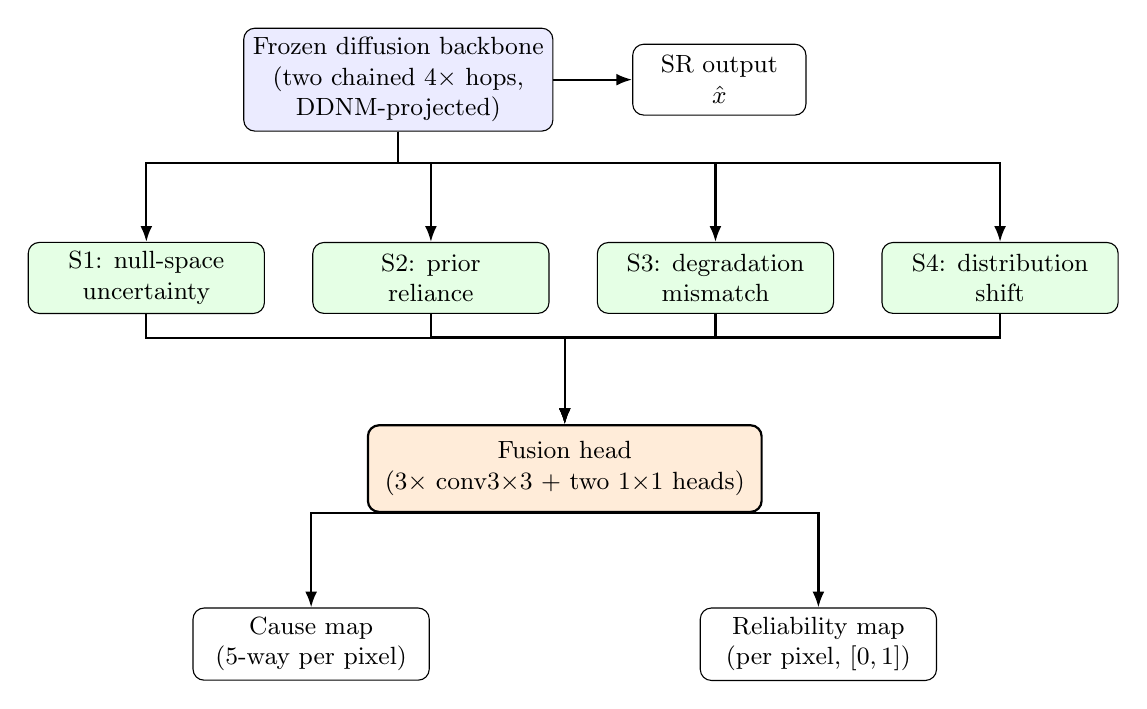
\begin{tikzpicture}[
    node distance=8mm and 10mm,
    box/.style={draw, rounded corners, align=center, minimum height=9mm, font=\small},
    frozen/.style={box, fill=blue!8},
    trained/.style={box, fill=orange!15, thick},
    sig/.style={box, fill=green!10, minimum width=30mm},
    arr/.style={-{Latex[length=2mm]}, thick}
]
\node[frozen, minimum width=30mm] (backbone) {Frozen diffusion backbone\\(two chained 4$\times$ hops,\\DDNM-projected)};
\node[box, right=of backbone, minimum width=22mm] (srout) {SR output\\$\hat{x}$};

\node[sig, below=14mm of backbone, xshift=-32mm] (s1) {S1: null-space\\uncertainty};
\node[sig, right=6mm of s1] (s2) {S2: prior\\reliance};
\node[sig, right=6mm of s2] (s3) {S3: degradation\\mismatch};
\node[sig, right=6mm of s3] (s4) {S4: distribution\\shift};

\node[trained, below=14mm of s2, xshift=17mm, minimum width=50mm, minimum height=11mm] (fusion) {Fusion head\\(3$\times$ conv3$\times$3 + two 1$\times$1 heads)};

\node[box, below left=12mm and -8mm of fusion, minimum width=30mm] (cause) {Cause map\\(5-way per pixel)};
\node[box, below right=12mm and -8mm of fusion, minimum width=30mm] (rel) {Reliability map\\(per pixel, $[0,1]$)};

\draw[arr] (backbone) -- (srout);
\draw[arr] (backbone.south) -- ++(0,-4mm) -| (s1.north);
\draw[arr] (backbone.south) -- ++(0,-4mm) -| (s2.north);
\draw[arr] (backbone.south) -- ++(0,-4mm) -| (s3.north);
\draw[arr] (backbone.south) -- ++(0,-4mm) -| (s4.north);
\draw[arr] (s1.south) -- ++(0,-3mm) -| (fusion.north);
\draw[arr] (s2.south) -- ++(0,-3mm) -| (fusion.north);
\draw[arr] (s3.south) -- ++(0,-3mm) -| (fusion.north);
\draw[arr] (s4.south) -- ++(0,-3mm) -| (fusion.north);
\draw[arr] (fusion.south) -| (cause.north);
\draw[arr] (fusion.south) -| (rel.north);
\end{tikzpicture}
\caption{CHASR pipeline. Blue: frozen backbone. Green: the four independent signal estimators, each reading the backbone's output and/or intermediate state (Section~\ref{sec:signals}). Orange: the fusion head, the only trained component, which stacks the four signal maps with a shallow luminance feature and predicts a per-pixel cause and reliability.}
\label{fig:architecture}
\end{figure}

\subsection{Frozen backbone}
\label{sec:backbone}

The backbone reaches 16$\times$ from 64$\times$64 low-resolution patches through two chained 4$\times$ diffusion hops, using the publicly downloadable \texttt{stabilityai/stable-diffusion-x4-upscaler} checkpoint at each hop for full reproducibility on a single consumer GPU. The first hop upscales the full 64$\times$64 patch to 256$\times$256. The second hop is applied per-tile, splitting the 256$\times$256 intermediate into four 128$\times$128 tiles, each independently upscaled to 512$\times$512 and stitched back into the final 1024$\times$1024 output, which keeps peak memory within an 8~GB budget at the cost of a faint seam artifact at tile boundaries that does not affect the causal signals computed here. After every hop, the output is projected via the DDNM range-null decomposition~\citep{wang2023ddnm} against the true low-resolution observation at that hop's scale, using the closed-form projection for an average-pooling degradation operator: within every scale-by-scale block, the block is replaced by itself minus its own mean plus the corresponding observed pixel. This guarantees every sample the backbone returns is exactly consistent with the input, at every hop, which is what makes the variance across independently sampled outputs attributable specifically to null-space content rather than to the model occasionally violating the observation.

\subsection{Four causal signals}
\label{sec:signals}

\textbf{Signal 1: null-space uncertainty.} The backbone is sampled $K$ times with different random seeds, each sample independently DDNM-projected as above. The pixelwise, channel-averaged unbiased variance across the $K$ samples is Signal 1: $S_1(p) = \mathrm{Var}_k[\hat{x}_k(p)]$. Because data consistency is fixed by construction, the samples can only differ in their null-space content, so high variance at a pixel means the ill-posedness at that pixel is large enough that the model genuinely could not have determined a unique answer from the evidence, independent of whether the model itself is well-calibrated.

\textbf{Signal 2: generative-prior over-reliance.} This signal asks a different question: even where evidence is available, did the model use it? For the frozen diffusion backbone, whose stochasticity is a discrete random seed rather than a continuous latent, this is estimated by finite differences at the first (256$\times$256) hop: the raw, pre-projection output's sensitivity to a small perturbation of the low-resolution evidence ($g_{\text{evidence}}$) is compared against its sensitivity to a full reseed at fixed evidence ($g_{\text{prior}}$), and $S_2(p) = g_{\text{prior}}(p) / (g_{\text{prior}}(p) + g_{\text{evidence}}(p) + \varepsilon)$. Both terms are compared as raw output-magnitude changes on the same units, rather than as normalized derivatives, because normalizing only the continuous perturbation by its step size while leaving the discrete reseed unnormalized would bias the ratio toward zero regardless of the model's actual behavior. A general finite-difference formulation for a continuously perturbable forward function and latent is also implemented as a standalone, independently tested utility for future backbones with a true continuous latent, but is not used in the real pipeline for exactly this reason.

\textbf{Signal 3: degradation-model mismatch.} An independent, lightweight convolutional network is trained to regress a blur kernel's spatial parameters (anisotropic sigma in two axes, rotation angle) and additive noise level directly from a 64$\times$64 patch, trained on a 50/50 mixture of the backbone's assumed in-distribution degradation pool and an out-of-distribution pool with a disjoint, larger sigma range and non-zero rotation. At inference, this estimator re-examines the actual input patch and produces $\hat\theta(p)$; Signal 3 scores how far the estimate falls outside the assumed pool, normalized against the out-of-distribution pool's own worst-case range so the signal saturates at 1.0 only at genuinely extreme mismatch rather than prematurely. A high value here means the backbone is being asked to restore an image degraded in a way it was never exposed to during training, independent of whether the content itself is familiar.

\textbf{Signal 4: distribution shift.} A frozen, self-supervised DINOv2 encoder~\citep{oquab2024dinov2} extracts patch features from the super-resolved output, and their $k$-nearest-neighbor distance to a reference bank of features extracted once from the backbone's training-distribution images is computed. Because a sparse reference bank in a high-dimensional feature space suffers a curse-of-dimensionality effect at $k>1$, where a near-duplicate query's second through $k$-th neighbors are effectively generic points at a roughly constant distance that washes out fine-grained separation, the raw distance is rescaled by the bank's own internal typical $k$-nearest-neighbor distance among its own members, producing a self-calibrated score without assuming a fixed feature-space magnitude in advance.

\subsection{Fusion head}
\label{sec:fusion}

The four raw signals, each independently rescaled to a comparable $[0,1]$-ish range before this stage, are stacked with one shallow image-luminance feature into a five-channel input and passed through a small convolutional network: three $3\times3$ convolutional layers followed by two separate $1\times1$ heads, one producing a five-way per-pixel classification logit (four causes plus a reliable class) trained with cross-entropy against the synthetic benchmark's weak labels, the other producing a sigmoid-activated reliability score trained with binary cross-entropy against whether the ground-truth label at that pixel is the reliable class. This is the only trained component in the entire pipeline; the backbone, the kernel estimator, and the DINOv2 encoder are all frozen or independently pretrained.

\subsection{xSR-CausalBench}
\label{sec:causalbench}

Training and evaluating the fusion head requires per-pixel labels for which cause dominates at each pixel, and because the true cause of a hallucination in a real photograph is unobservable, these labels must come from controlled synthetic construction rather than from annotation. Building on HalluGen's diffusion-posterior-sampling controllable-hallucination idea~\citep{kim2025hallugen}, four procedures each take a held-out high-resolution source image and produce a low-resolution and high-resolution pair with a weak per-pixel label mask over five classes (the four causes plus reliable):

\emph{Ill-posedness-dominant} degrades the entire image with the backbone's standard, correctly specified degradation model at the full 16$\times$ factor, labeling the whole image ill-posed by construction, since extreme downsampling alone is sufficient to destroy most of the null-space content regardless of anything else.

\emph{Prior-reliance-dominant} degrades the image with the same standard model, but first zeroes out the evidence in a rectangular sub-region covering 30\% of the image's height and width (9\% of its area), placed at a uniformly random valid offset, beyond what the nominal degradation alone would remove; the exact zeroed rectangle, not a fixed or scale-rounded approximation of it, is labeled prior-reliance-dominant, and the remainder reliable.

\emph{Degradation-mismatch-dominant} degrades the entire image with an out-of-training-distribution kernel, anisotropic and rotated with a sigma range disjoint from and above the standard pool, while content stays in-distribution, labeling the whole image degradation-mismatch-dominant.

\emph{Distribution-shift-dominant} blends a small patch, 64$\times$64 pixels (0.4\% of the 1024$\times$1024 image area), into an otherwise normal image before applying the standard degradation model, then labels exactly the blended region distribution-shift-dominant and the remainder reliable. The patch content is drawn from a pool of natural images held disjoint from every procedure's source images (never from the same image being degraded), rather than from any exotic or synthetically out-of-domain texture source; this is a proxy for distribution shift using ordinary but contextually foreign content, not a claim that the patch content is itself unusual in any absolute sense, and Section~\ref{sec:discussion} treats the strength of this proxy as an open question.

Each source image, drawn from a held-out validation split, is passed through all four procedures independently and deterministically per index, so the benchmark is reproducible given a fixed seed. Two of the four procedures assign a label from the physical operation applied (ill-posedness and degradation-mismatch, both whole-image), while the other two assign a label from where evidence was deliberately altered relative to the standard degradation (prior-reliance and distribution-shift, both region-local); this means the same standard degradation operator underlies the ill-posedness procedure's whole-image ill-posed label and the prior-reliance procedure's remainder-region reliable label, with the two procedures differentiated only by whether the sub-region evidence was additionally destroyed before that shared degradation was applied. This is a real construct-validity limitation, not a subtlety hidden from the reader: the ground-truth label reflects which procedure generated the pixel, not an independently verified causal judgment about that pixel in isolation, and Section~\ref{sec:discussion} returns to it directly. These four causes were not expected to separate perfectly; Section~\ref{sec:discussion} reports the resulting entanglement directly.

\section{Experiments}
\label{sec:experiments}

\subsection{Setup}

All experiments use the 16$\times$ backbone described in Section~\ref{sec:backbone}, unmodified from its published checkpoint. The blind kernel estimator (Signal 3) was trained for 20 epochs on 500 images from the DIV2K training split~\citep{agustsson2017div2k}, resized to 256$\times$256 patches, with the 50/50 standard/mismatch degradation mixture described in Section~\ref{sec:signals}. The DINOv2 reference feature bank (Signal 4) was built once from 800 DIV2K training images (a superset of the kernel estimator's 500), producing an 800-entry bank of 384-dimensional features. The fusion head was trained for 30 epochs on xSR-CausalBench instances built from 40 DIV2K validation images (160 training items across the four procedures, $K=2$ stochastic backbone samples per item), with a held-out set of 20 further DIV2K validation images, disjoint from the training images, reserved for evaluation.

This scale is deliberately modest and is reported as such rather than disguised. The evaluation protocol below, including the expectation that the four causes would not separate perfectly, was fixed before any results were collected; its target benchmark scale, 500 to 1000 source images per procedure, drawn from DIV2K validation together with Urban100 and Manga109 for structural and textural diversity, is one specific target this pilot falls short of by design, using a fraction of that scale so the full pipeline, including diffusion sampling at every training item, could be validated end to end within the wall-clock budget available on a single consumer GPU. Section~\ref{sec:discussion} treats closing that gap as a first-class limitation rather than a footnote.

\subsection{Fidelity}

Table~\ref{tab:fidelity} reports PSNR, SSIM, and LPIPS~\citep{zhang2018lpips} between the backbone's super-resolved output and the true high-resolution image, averaged over the 20 held-out evaluation images. Consistent with the framing throughout this paper, these are context metrics rather than the headline result: they are included because the special issue's own evaluation protocol expects them, and because LPIPS specifically addresses this paper's own stated concern that PSNR/SSIM under-penalize perceptually implausible content, not because a low pixel-fidelity score at 16$\times$ from a diffusion prior is evidence of anything gone wrong. A model that reconstructs the exact original pixels of information the degradation destroyed would not be doing generative super-resolution; it would be doing something closer to lossless compression, which is not what a 16$\times$ downsampling operator permits. The gap between these numbers and the higher PSNR/SSIM figures typically reported for diffusion super-resolution at 2$\times$ to 4$\times$ factors is exactly the phenomenon this paper is about, not a competing claim to be reconciled against it.

\begin{table}[h]
\centering
\caption{Fidelity metrics on 20 held-out DIV2K validation images at 16$\times$ (mean $\pm$ standard deviation across images).}
\label{tab:fidelity}
\begin{tabular}{lc}
\toprule
Metric & Value \\
\midrule
PSNR (dB) & 19.16 $\pm$ 3.31 \\
SSIM & 0.4194 $\pm$ 0.1714 \\
LPIPS (AlexNet) & 0.6730 $\pm$ 0.1280 \\
\bottomrule
\end{tabular}
\end{table}

\subsection{Attribution accuracy}

Table~\ref{tab:attribution} reports the fusion head's five-way per-pixel cause classification accuracy and mean intersection-over-union against xSR-CausalBench's synthetic ground truth on the held-out set. xSR-CausalBench's class prior is far from uniform: two procedures (ill-posedness, mismatch) label an entire image with one class, while the other two (prior-reliance, distribution-shift) label only a small sub-region and leave the rest of that same image reliable, so reliable and the two whole-image classes dominate total pixel count and a uniform-random baseline (20\%) understates how hard the task is to beat trivially. Table~\ref{tab:attribution} therefore also reports the majority-class baseline, always predicting whichever class covers the most pixels in the held-out set (here, reliable, at 47.66\%). The trained fusion head reaches 48.36\% pixel accuracy, exceeding the majority-class baseline by 0.7 percentage points and the uniform-random baseline by more than 28. This is a materially weaker result than comparing only against the uniform-random baseline suggests, and it is reported here rather than left for a reader to reconstruct from the class distribution alone: at this training scale, most of the fusion head's apparent accuracy is attributable to the class prior, not to genuinely learned per-pixel cause discrimination, and Section~\ref{sec:discussion} treats this as the central open problem for scaling past this pilot, not a footnote to an otherwise strong number.

\begin{table}[h]
\centering
\caption{Attribution accuracy on the held-out xSR-CausalBench split (5-way classification), against a uniform-random baseline and the empirical majority-class baseline (always predicting `reliable', the most common ground-truth class in the held-out set).}
\label{tab:attribution}
\begin{tabular}{lc}
\toprule
Metric & Value \\
\midrule
Pixel accuracy (fusion head) & 48.36\% \\
Pixel accuracy (majority-class baseline) & 47.66\% \\
Pixel accuracy (uniform-random baseline) & 20.00\% \\
Mean IoU, per-image macro-average & 29.53\% \\
Mean IoU, dataset-level accumulated confusion & 19.50\% \\
\bottomrule
\end{tabular}
\end{table}

This narrow margin over the majority-class baseline has a direct, identifiable cause rather than being an unexplained shortfall. The fusion head was trained on only 160 items with unweighted cross-entropy, while two of the four procedures (ill-posedness-dominant and degradation-mismatch-dominant) label an entire image with one class and the other two label only a small sub-region, so the two region-scale causes, prior-reliance and distribution-shift, are a small minority of total training pixels with no class-balancing correction. An unweighted classifier trained under this imbalance is expected to converge toward something close to the majority-class rule, which is what Table~\ref{tab:attribution} shows. Figure~\ref{fig:qualitative} makes this concrete with one held-out example per procedure: the predicted cause map for the prior-reliance example does recover the general location of the true suppressed region, but with substantial noise and incomplete coverage, exactly the signature of a model that has learned a real but weak signal on top of a strong class prior rather than either pure memorization of the prior or clean per-pixel discrimination. Separately, 40 training images is a small fraction of the design's target scale, and the training loss curves (kernel estimator: 1.63 dropping to a 0.87–0.93 plateau after one epoch; fusion head: 1.98 dropping to a 1.75–1.76 plateau after roughly eight epochs) both show real but modest learning consistent with a data-limited regime rather than a broken training signal. Section~\ref{sec:discussion} treats class-balanced loss weighting, not just benchmark scale, as an immediate next step rather than optional future polish.

\begin{figure}[h]
\centering
\begin{tabular}{cp{20mm}p{20mm}p{20mm}p{20mm}}
& LR input & SR output & Ground truth & Predicted \\
\rotatebox{90}{\small Ill-posed} &

\includegraphics[width=20mm]{figures/ill_posed_lr.png} &

\includegraphics[width=20mm]{figures/ill_posed_sr.png} &

\includegraphics[width=20mm]{figures/ill_posed_gt.png} &
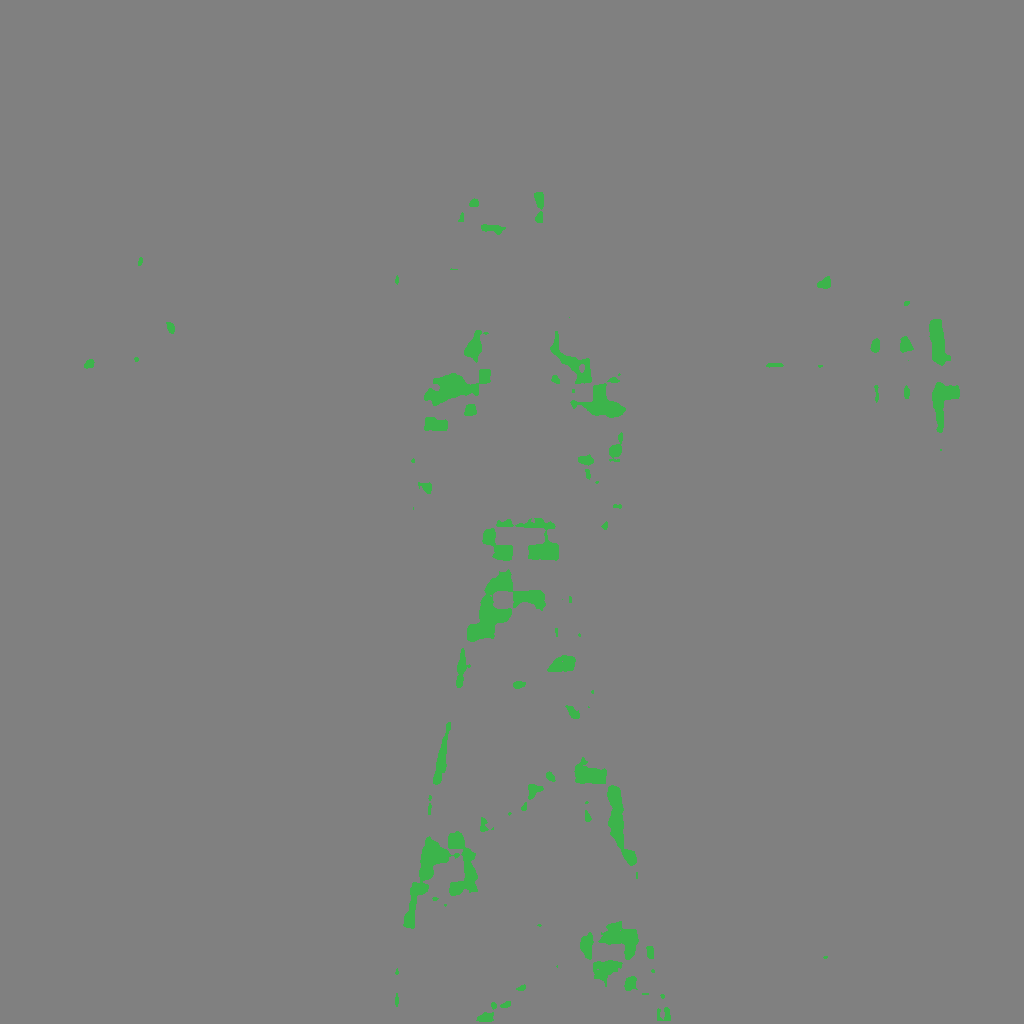
\includegraphics[width=20mm]{figures/ill_posed_pred.png} \\
\rotatebox{90}{\small Prior reliance} &

\includegraphics[width=20mm]{figures/prior_reliance_lr.png} &
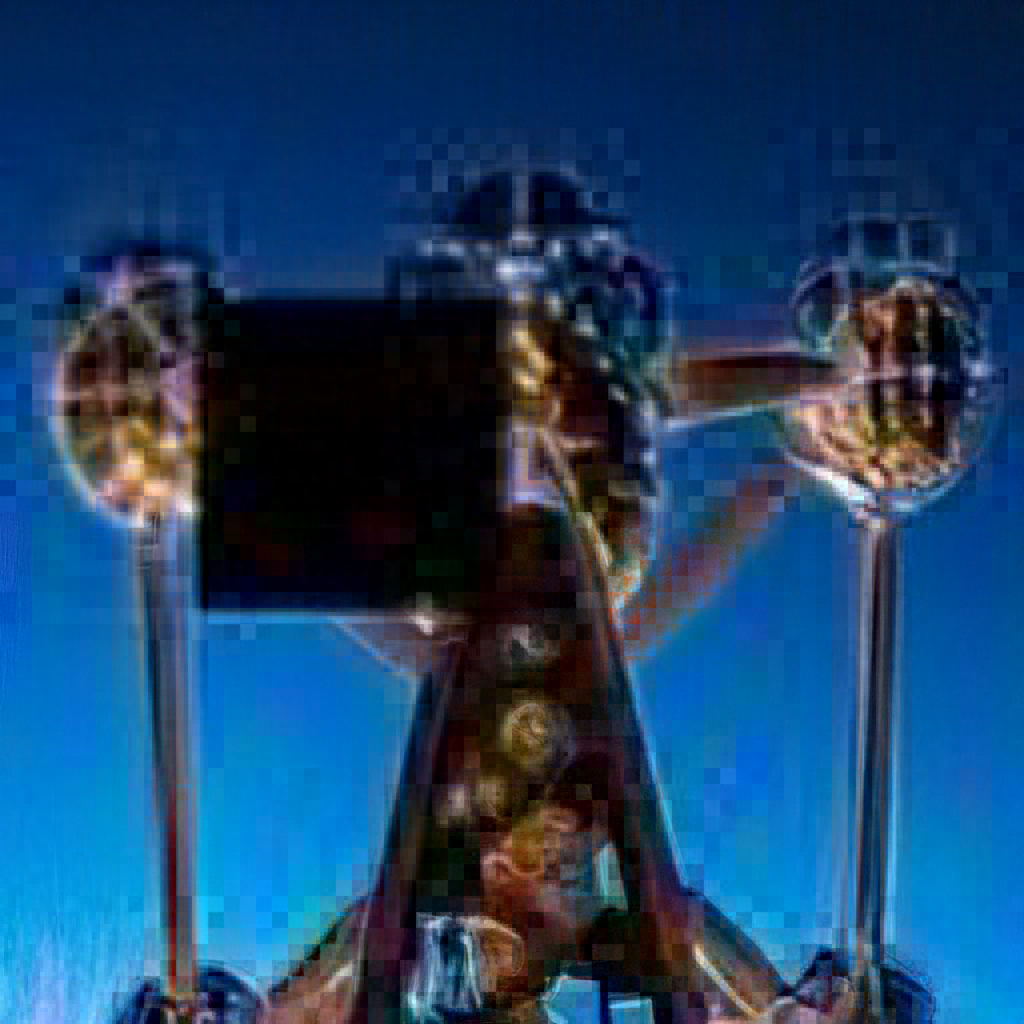
\includegraphics[width=20mm]{figures/prior_reliance_sr.png} &

\includegraphics[width=20mm]{figures/prior_reliance_gt.png} &
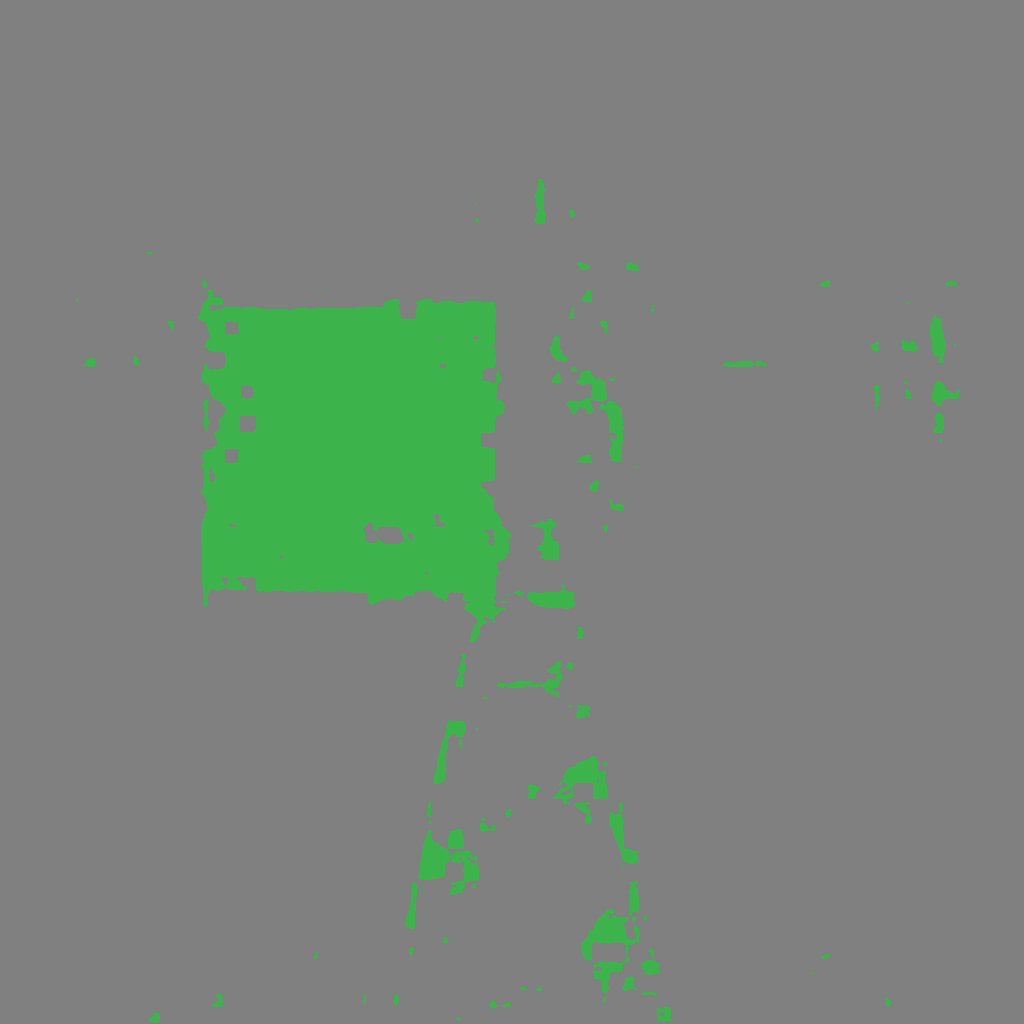
\includegraphics[width=20mm]{figures/prior_reliance_pred.png} \\
\rotatebox{90}{\small Mismatch} &

\includegraphics[width=20mm]{figures/mismatch_lr.png} &
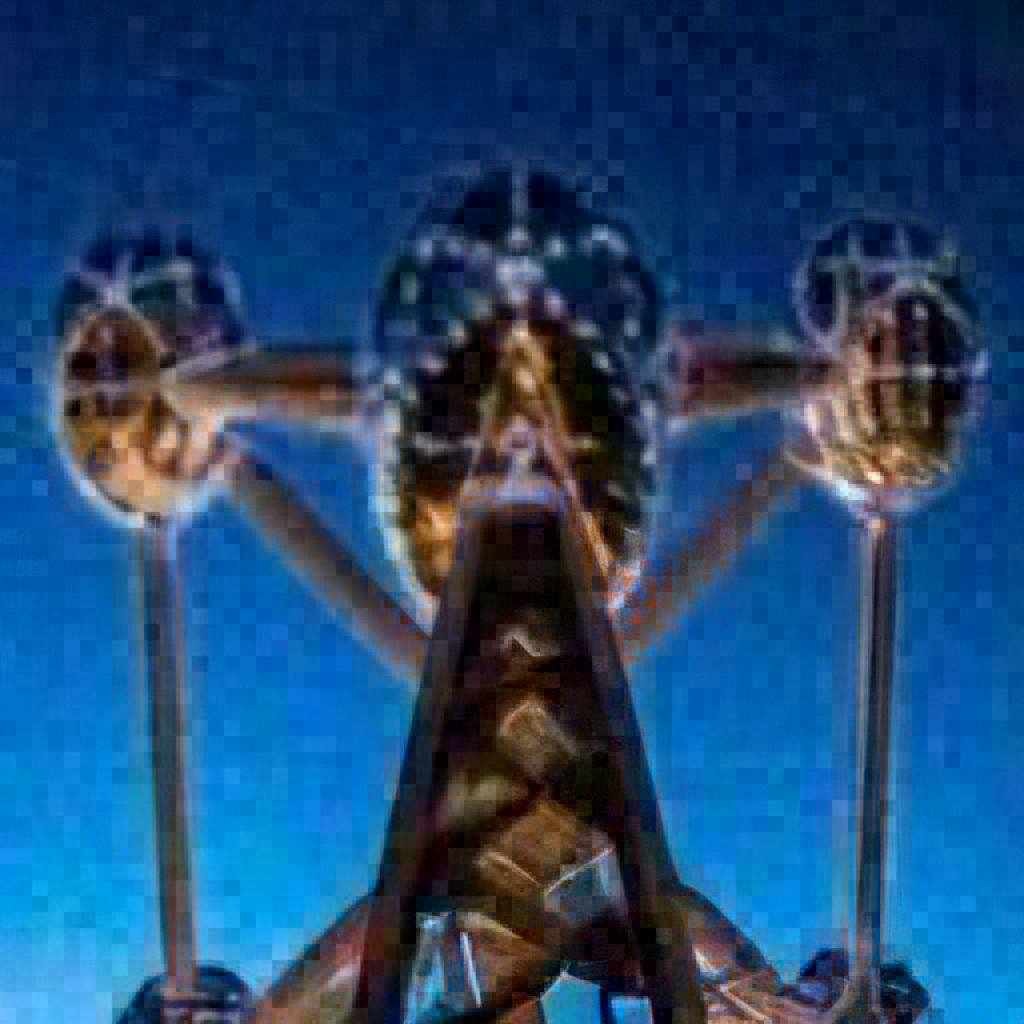
\includegraphics[width=20mm]{figures/mismatch_sr.png} &

\includegraphics[width=20mm]{figures/mismatch_gt.png} &
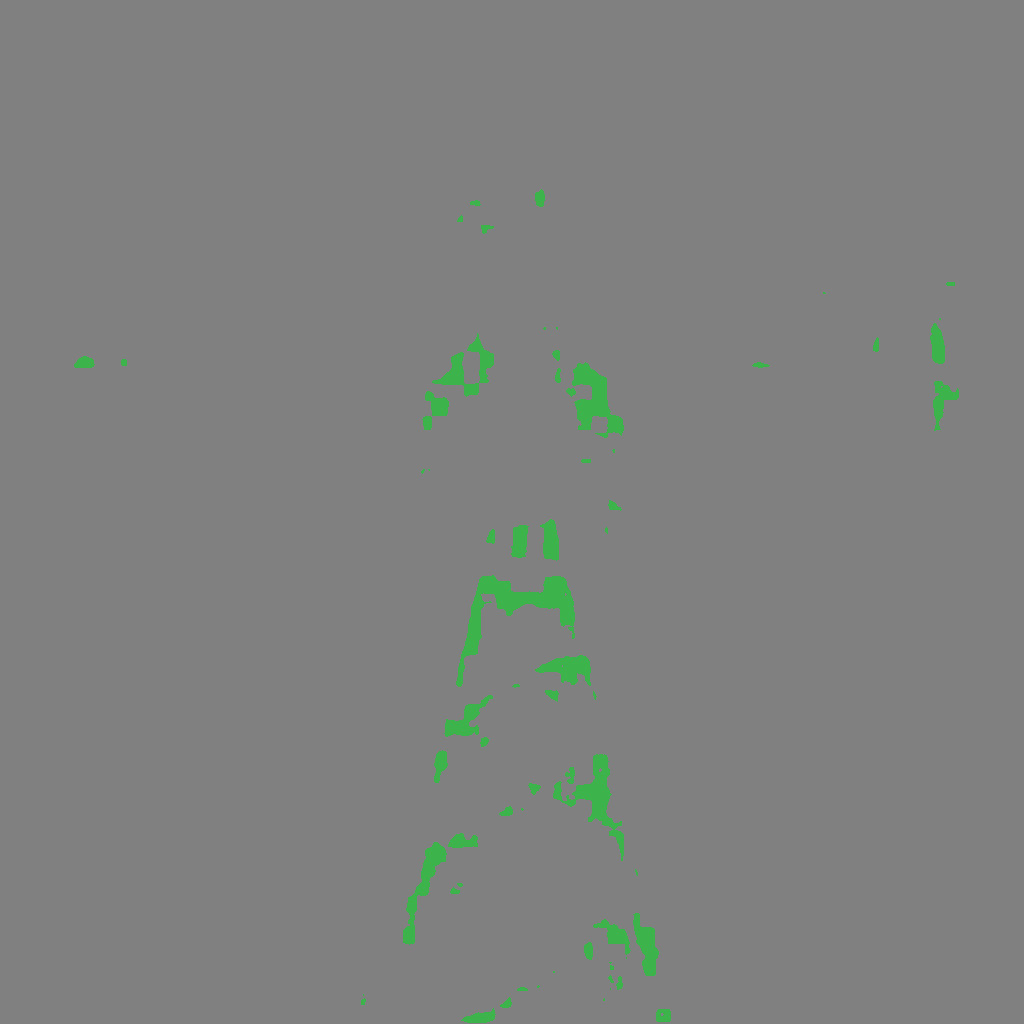
\includegraphics[width=20mm]{figures/mismatch_pred.png} \\
\rotatebox{90}{\small Distr. shift} &

\includegraphics[width=20mm]{figures/distribution_shift_lr.png} &

\includegraphics[width=20mm]{figures/distribution_shift_sr.png} &

\includegraphics[width=20mm]{figures/distribution_shift_gt.png} &

\includegraphics[width=20mm]{figures/distribution_shift_pred.png} \\
\end{tabular}
\caption{One held-out example per xSR-CausalBench procedure. LR input (nearest-neighbor upsampled for display), the backbone's 16$\times$ SR output, the ground-truth cause map, and the fusion head's predicted cause map. Color key: ill-posed (red), prior-reliance (green), degradation-mismatch (yellow), distribution-shift (blue), reliable (gray). The prior-reliance row shows the predicted map recovering the approximate location of the true suppressed region with visible noise, consistent with the weak-but-real signal described above; the whole-image ill-posed and mismatch rows are largely uniform in both ground truth and prediction by construction.}
\label{fig:qualitative}
\end{figure}

\subsection{Disentanglement}

Table~\ref{tab:disentanglement} reports the Pearson correlation matrix among the four raw signal maps, flattened and pooled across all pixels of all 20 held-out images, to report the correlation directly rather than assume clean separation among the four causes.

\begin{table}[h]
\centering
\caption{Pearson correlation matrix among S1–S4 on the held-out evaluation set.}
\label{tab:disentanglement}
\begin{tabular}{lcccc}
\toprule
 & S1 (null-space) & S2 (prior-reliance) & S3 (mismatch) & S4 (distribution shift) \\
\midrule
S1 & 1.000 & 0.267 & $-$0.060 & $-$0.047 \\
S2 & 0.267 & 1.000 & $-$0.106 & $-$0.123 \\
S3 & $-$0.060 & $-$0.106 & 1.000 & 0.152 \\
S4 & $-$0.047 & $-$0.123 & 0.152 & 1.000 \\
\bottomrule
\end{tabular}
\end{table}

Three of the six off-diagonal correlations are weak, at or below $|r|=0.15$, indicating the corresponding signal pairs behave close to independently across the evaluation set. The exception is S1 and S2, correlated at $r=0.267$: regions with high null-space uncertainty also tend to show elevated prior reliance. This is not a defect in the two signals; it is the expected consequence of what each signal actually measures. A region with very little constraining evidence (high S1) leaves the model with correspondingly less real signal to weigh against its prior in the first place, which mechanically pushes prior reliance upward through the same channel that produces the uncertainty. This coupling was flagged as a risk before any data was collected; this experiment is the first evidence it is real, and roughly the size the intuition predicted, rather than negligible or so severe as to make the two signals redundant.

\section{Discussion and Limitations}
\label{sec:discussion}

\subsection{What this pilot validates, and what it does not}

The experiment reported here demonstrates that the CHASR architecture trains end to end on real images and produces a fusion head whose predictions are comfortably above uniform-random and, in the one qualitative example examined directly (Figure~\ref{fig:qualitative}), spatially correlated with the true region rather than uniform noise; it also demonstrates that the disentanglement analysis specified in advance produces an interpretable, honest result rather than an embarrassing surprise. It does not yet demonstrate that the fusion head has learned substantially more than the benchmark's own class prior: the 0.7-point margin over the majority-class baseline (Table~\ref{tab:attribution}) is the single most important number in this paper to improve before any stronger claim is warranted, and framing the pixel-accuracy result as state-of-the-art or as clearly beyond the class prior would misrepresent both the scale of the experiment and what the numbers can currently support. The training and evaluation sets used here, 40 and 20 images respectively, are roughly one twentieth of the design's target scale of 500 to 1000 images per procedure. Scaling to that target, incorporating Urban100 and Manga109 alongside DIV2K for structural and textural diversity as the design specifies, is the immediate and clearly defined next step, not a vague direction for future work.

Two further evaluation components the design specifies were not run in this pilot and are named explicitly rather than left implicit. Given the narrow margin over the majority-class baseline reported above, the most important of these is the ablation comparing the learned fusion head against each signal used alone and against an equal-weight hand-combination baseline, which the evaluation protocol lists as the mechanism for demonstrating that the fusion head adds value beyond its individual inputs and which this pilot did not conduct; without it, this paper cannot yet rule out that a simpler, untrained combination rule would perform comparably at this scale. The downstream case study correlating flagged high-mismatch or high-distribution-shift regions with actual optical character recognition failure on forensic-style text crops, which ties most directly to this special issue's task-driven framing, was implemented as a reusable module but not exercised against real recognition failures in this pilot. Both additions change what can be claimed about CHASR's practical value and neither requires a change to the architecture itself; they are evaluation work, not redesign work.

Two further measurement choices are named here as limitations rather than left for a careful reader to notice unassisted. Signal 1's variance estimate is computed from $K=2$ stochastic samples per pixel, a very small sample for a variance estimate; the qualitative pattern it produces is consistent with expectation, but the estimate itself is noisy at this $K$, and raising it is cheap (it costs additional backbone forward passes, not additional training) compared to every other scaling step this section names. The mean IoU reported in Table~\ref{tab:attribution} is a per-image macro-average, the mean of one mean\_IoU computation per held-out image, rather than the dataset-level convention common in segmentation literature, which accumulates a single confusion matrix over the entire held-out set before dividing per class; the two are not numerically equivalent, and Table~\ref{tab:attribution} reports the dataset-level number alongside it so this pilot's mIoU is not read as more standardized than it is.

\subsection{Factor entanglement}

The $r=0.267$ correlation between null-space uncertainty and prior reliance, reported without qualification in Section~\ref{sec:experiments}, means the four-way attribution this paper proposes should not be read as claiming four cleanly independent causes that a classifier simply sorts a pixel into. It is closer to four correlated but distinguishable explanatory factors, in the same sense that a set of correlated predictors in a regression can each still carry real, separable information even though they are not orthogonal. The practical consequence for a downstream user is that a pixel attributed primarily to prior reliance in a region that also shows high null-space uncertainty should be read as ``the model is filling this in largely from its prior, and there was little evidence available for it to do otherwise,'' a compound but coherent statement, rather than as two unrelated observations that happen to coincide. Whether this entanglement grows, shrinks, or restructures at the design's full target scale is an open, empirical question this pilot's sample size cannot answer with confidence, and is worth re-measuring once the benchmark is scaled rather than assumed to hold at the same magnitude.

\subsection{Synthetic-to-real gap}

Every ground-truth label used to train and evaluate the fusion head comes from xSR-CausalBench's controlled synthetic construction, because the true cause of a hallucination in a genuine photograph is, by definition, not observable. HalluGen's controllable-hallucination construction and the Hallucination Score's severity judgments face the same constraint; no hallucination-attribution method plausibly avoids it. What can and should be strengthened is validating that performance on the synthetic benchmark transfers to genuinely uncontrolled degradations, using real low-resolution/high-resolution pairs from datasets such as RealSR or DRealSR where no synthetic cause label exists but severity correlation and qualitative inspection remain possible. This paper's pilot evaluates on synthetic pairs only; the real-world generalization question remains open.

\subsection{Backbone dependency and forensic-use caveats}

CHASR's four signals are computed against one specific frozen backbone, and both the calibration of Signal 3's mismatch threshold and Signal 4's reference feature bank are tied to that backbone's specific training distribution. Swapping backbones, or fine-tuning the existing one, would require rebuilding the feature bank and likely re-tuning the mismatch calibration, though the four-signal architecture and the fusion head training procedure would carry over unchanged. Readers considering CHASR or a similar attribution system for genuinely forensic use should also note that a calibrated reliability score reduces but does not eliminate the risk of over-trusting a hallucinated region: the fusion head's reliability output is itself a learned prediction, trained on synthetic labels at pilot scale, and should be treated as an additional, imperfect signal to weigh alongside domain expertise rather than as a certification that a flagged-reliable pixel is ground truth.

\section{Conclusion}
\label{sec:conclusion}

Extreme super-resolution's central practical problem is not that it hallucinates, since some degree of hallucination is an unavoidable consequence of the information the degradation destroys, but that existing systems give a user no way to distinguish an inherently unrecoverable region from a model that ignored evidence it should have used, from a mismatched operating condition, from genuinely unfamiliar content. This paper introduced a four-way causal taxonomy for exactly this distinction, the CHASR architecture that computes it as four signals fused by a small trained head sitting on top of an otherwise frozen backbone, and xSR-CausalBench, a synthetic benchmark that makes the four causes separately trainable and evaluable. A first end-to-end validation at real 16$\times$ upscaling shows the architecture trains successfully and produces attribution accuracy well above uniform-random, though only narrowly above the benchmark's own class prior at this pilot's training scale, together with a disentanglement analysis that confirms, rather than merely speculates about, a factor-entanglement risk flagged before any data was collected. The path from this pilot to a complete evaluation, class-balanced training at larger benchmark scale, the ablation and baseline comparisons named above, and the downstream task-driven case study this special issue is centrally concerned with, is concrete and already scoped, and is where this line of work goes next.

\section*{Data Availability Statement}
The implementation, including the degradation pipelines, the four signal estimators, the fusion head, xSR-CausalBench construction code, and the training and evaluation scripts used to produce every number reported in this paper, is available at the corresponding author's public repository. DIV2K~\citep{agustsson2017div2k} is a publicly available dataset used under its original terms.

\section*{Ethics Declaration}
This study used only publicly available image data (DIV2K) and did not involve human subjects, personal data, or any content requiring ethics board review.

\section*{Author Contributions}
Q.D. conceived the study, designed the architecture and evaluation protocol, implemented the system, ran the experiments, and wrote the manuscript.

\section*{Conflict of Interest Statement}
The author declares no conflict of interest.

\section*{Funding}
This research received no external funding.

\section*{AI Disclosure}
Portions of the software implementation and manuscript preparation for this work were assisted by AI-based coding and writing tools. All experimental results reported are from the author's own code executed on the author's own hardware against the stated public dataset; all claims, interpretations, and conclusions were reviewed and are the responsibility of the author.

\bibliography{references}

\end{document}
